% !TEX root= ../main.tex
\subsection{Discourse Theories and Digraphs}
\label{sub:Discourse Theories and Digraphs}
As mentioned earlier, there is a close connection between (1) models of a discourse theory, (2) kernels of a graph and (3) solutions of a graph.
While Roy Cook has given us the equality of (2) and (3), we will now look at two functions connecting (1) and (2).  We get the following definitions from \cite{}

$\mathcal{T}:$ translating a digraph \textbf{G} into a corresponding theory $\mathcal{T}(\mathbf{G})$ such that $sol(\mathbf{G}) = mod(\mathcal{T}(G))$.

$\mathcal{G}:$ translating a theory $T$ into a corresponding digraph $\mathcal{G}(T)$ such that $mod(T) = sol(\mathcal{G}(T))$.

Given any digraph \textbf{G} we get the theory $\mathcal{T}(\mathbf{G})$ by taking, for each $x \in G$, the formula $x \leftrightarrow \bigwedge_{y \in N(x)} \neg y$ where $\bigwedge \emptyset = 1$.\\

\begin{example}
  \[
    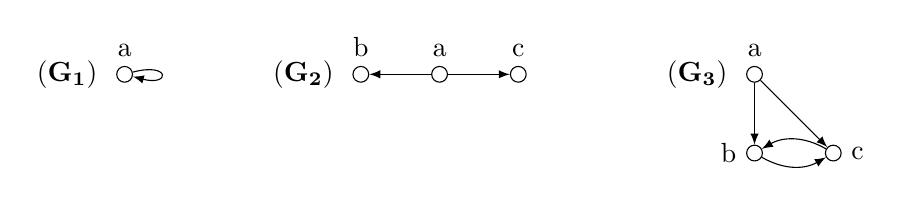
\begin{tikzpicture}
      [
      point/.style={circle,draw,inner sep=0pt,minimum size=2mm},
      collection/.style={thick,rectangle,draw,inner sep=0pt,minimum height=14mm, minimum width= 9mm}
      ]
      \node (label) at (0,1) [label=left:$(\mathbf{G_1})\;$] {};
      \node (0) at (0,1) [point,label=above:a] {};
      \draw [-latex, loop right] (0) to (0);

      \node (label) at (3,1) [label=left:$(\mathbf{G_2})\;$] {};
      \node (0) at (4,1) [point,label=above:a] {};
      \node (1) at (3,1) [point,label=above:b] {};
      \node (2) at (5,1) [point,label=above:c] {};
      \draw [-latex] (0) to (1);
      \draw [-latex] (0) to (2);

      \node (label) at (8,1) [label=left:$(\mathbf{G_3})\;$] {};
      \node (0) at (8,1) [point,label=above:a] {};
      \node (1) at (8,0) [point,label=left:b] {};
      \node (2) at (9,0) [point,label=right:c] {};
      \draw [-latex] (0) to (2);
      \draw [-latex] (0) to (1);
      \draw [-latex, bend right] (1) to (2);
      \draw [-latex, bend right] (2) to (1);
    \end{tikzpicture}
  \]
  Using the graphs from above, we get the following theories using $\mathcal{T}$:
  \begin{align}
    \mathcal{T}(\mathbf{G_1}) &= \big \{ a \leftrightarrow \neg a \big \} \\
    \mathcal{T}(\mathbf{G_2}) &= \big \{ a \leftrightarrow (\neg b \wedge \neg c), b, c \big \}\\
    \mathcal{T}(\mathbf{G_3}) &= \big \{ a \leftrightarrow (\neg b \wedge \neg c), b \leftrightarrow \neg c, c \leftrightarrow \neg b \big \}
  \end{align}
\end{example}
We will not be proving that $sol(\mathbf{G}) = mod(\mathcal{T}(G))$, but observe that $\mathbf{G_1}$ has no solution, just like its corresponding theory $\mathcal{T}(\mathbf{G_1})$ has no satisfying models.
$\mathbf{G_2}$ has one solution, where one assigns $a=0, b=1, c=1$.
This assignment also works as a satisfying model for $\mathcal{T}(\mathbf{G_2})$.
In $\mathbf{G_3}$, we get two solutions, both with $a$ assigned to 0, but with 0 and 1 distributed on $b$ and $c$.
These are also the only two models satisfying $\mathcal{T}(\mathbf{G_3})$.
It is generally true that $\mathcal{T}$ gives us our requested correspondence.

Conversely, given any discourse theory $T$ (in fact, this will work given any PL theory, since we can translate CNF to GNF), we can derive the corresponding graph $\mathcal{G}(T)$ in the following way:
All variables in the theory are vertices, and for each formula $x \leftrightarrow \bigwedge_{i \in I_x} y_i$ make a directed edge $\langle x,y_i \rangle$ for each $i \in I_x$.\\

\begin{example}
  \begin{align}
    T_1 &= \neg a &&\iff ( a \lar \neg a'), (a' \lar \neg a), (y_1 \lar (\neg a' \wedge \neg y_1))\\
    T_2 &= a \vee b &&\iff ( a \lar \neg a'), (a' \lar \neg a), (b \lar \neg b'), (b' \lar \neg b), (y_1 \lar (\neg a \wedge \neg b \wedge \neg y_1))
  \end{align}
  Using $\mathcal{G}$ on the above theories -- translated to GNF -- gives us the following graphs:
  \[
    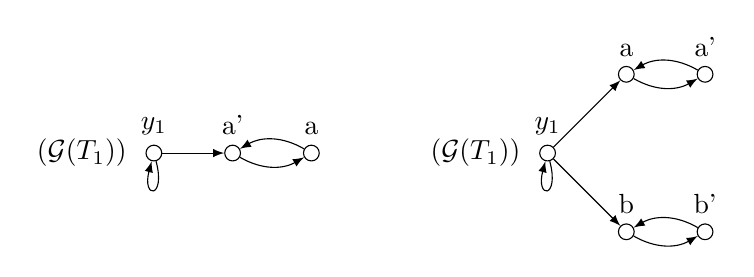
\begin{tikzpicture}
      [
      point/.style={circle,draw,inner sep=0pt,minimum size=2mm},
      collection/.style={thick,rectangle,draw,inner sep=0pt,minimum height=14mm, minimum width= 9mm}
      ]
      \node (label) at (0,1) [label=left:$(\mathcal{G}(T_1))\;$] {};
      \node (0) at (0,1) [point,label=above:$y_1$] {};
      \node (1) at (1,1) [point,label=above:a'] {};
      \node (2) at (2,1) [point,label=above:a] {};
      \draw [-latex, loop below] (0) to (0);
      \draw [-latex] (0) to (1);
      \draw [-latex, bend right] (1) to (2);
      \draw [-latex, bend right] (2) to (1);

      \node (label) at (5,1) [label=left:$(\mathcal{G}(T_1))\;$] {};
      \node (0) at (5,1) [point,label=above:$y_1$] {};
      \node (1) at (6,0) [point,label=above:b] {};
      \node (2) at (7,0) [point,label=above:b'] {};
      \node (3) at (6,2) [point,label=above:a] {};
      \node (4) at (7,2) [point,label=above:a'] {};
      \draw [-latex, loop below] (0) to (0);
      \draw [-latex] (0) to (1);
      \draw [-latex, bend right] (1) to (2);
      \draw [-latex, bend right] (2) to (1);
      \draw [-latex] (0) to (3);
      \draw [-latex, bend right] (3) to (4);
      \draw [-latex, bend right] (4) to (3);
    \end{tikzpicture}
  \]
  Again, will we not be proving the correspondence, but notice $T_1$ has one model satisfying it, where $a = 0$.
\end{example}
